\begin{document}
%=================================================================
%                           Start Document
%=================================================================
\setstretch{1.6}

\section{Discussion}
\lhead{Discussion} % section header
\subsection{Open Loop Sequence}
The results of the open loop FES highlighted the potential of sequence to produce consistent gait patterns, but there are several points that warrant discussion.
\newline

\textit{Testing in Healthy individuals}

One significant challenge is the inherent difficulty of testing FES on healthy subjects. Healthy individuals naturally recruit their muscles during walking, even when instructed to minimize voluntary muscle activity and rely on stimulation. This introduces variability in the response to FES, as the subjects neuromuscular system interacts with the stimulation in ways that differ from the intended clinical scenarios. These interaction can obscure the system's true efficacy.

There are also other possible consequences. Firstly, patients with neurological impairments, there might be less of a falling out of sync issue, which observed in healthy individual in this study. The lack of competing voluntary muscle activity could make FES-induced movements more consistent and predictable. Secondly, there is evidence suggesting that patients may perceive FES differently from healthy individuals. While healthy subject often report discomfort during stimulation, patients with neurological conditions may experience reduced discomfort, potentially making it easier to achieve functional movements. This could make the setup simpler and more comfortable and effective in patient populations. \todo{source}


\textit{Lack of Weight Support System}
Weight support could have created a more controlled environment for stimulation. Particularly in healthy individuals the it would have helped to minimize the effect of involuntary muscle contractions that all healthy individuals will have when placed on a treadmill. This would have lent more credibility to the results, as it is not certain how much of the movement during the gait is due only to the stimulation or if the subjects are inadvertently activating their muscles during the study.
\newline 

\textit{Alignment with Natural Synergies}

The gait sequence used in this study, while not explicitly modeled on natural synergies closely resembles the muscle synergies during normal gait. The primary deviation is in the absence of stimulation to the rectus femoris. In natural synergies, the rectus femoris plays a key role in both hip flection and knee extension \todo{source}. However, 

The decision to exclude rectus femoris stimulation was guided by the goal of creating a simple and comfortable sequence that is generalizable, not too complex to setup and applicable for clinical use. However, if the objective were to mimic the natural synergies, a low-current stimulation of the rectus femoris could be considered. Low current, since when stimulated it acts visibly as a knee extensor. This raises an important question about the trade offs between simplicity and fidelity to natural synergies, which should be be considered in the context of clinical goals.

\subsection{Knee Angle Extraction}

The results of the knee angle stimulation demonstrate that the In-House IMU-based estimation method, which utilizes an adapted Madgwick filter, performs effectively in estimating knee joint angles during movement. However, slight drift in the estimation was observed, despite the theoretical robustness of the Madgwick algorithm to such errors. This drift could be attributed to several factors the first of which is that the way in which the algorithm is implemented assumes that the local coordinate axes of the IMUs are perfectly aligned with the anatomical knee joint axis. Any misalignment introduces errors in the computed knee angle, as the algorithm assumes that the relative orientation of the two IMUs reflects the hinge joint's motion accurately.

\begin{figure}
    \centering
    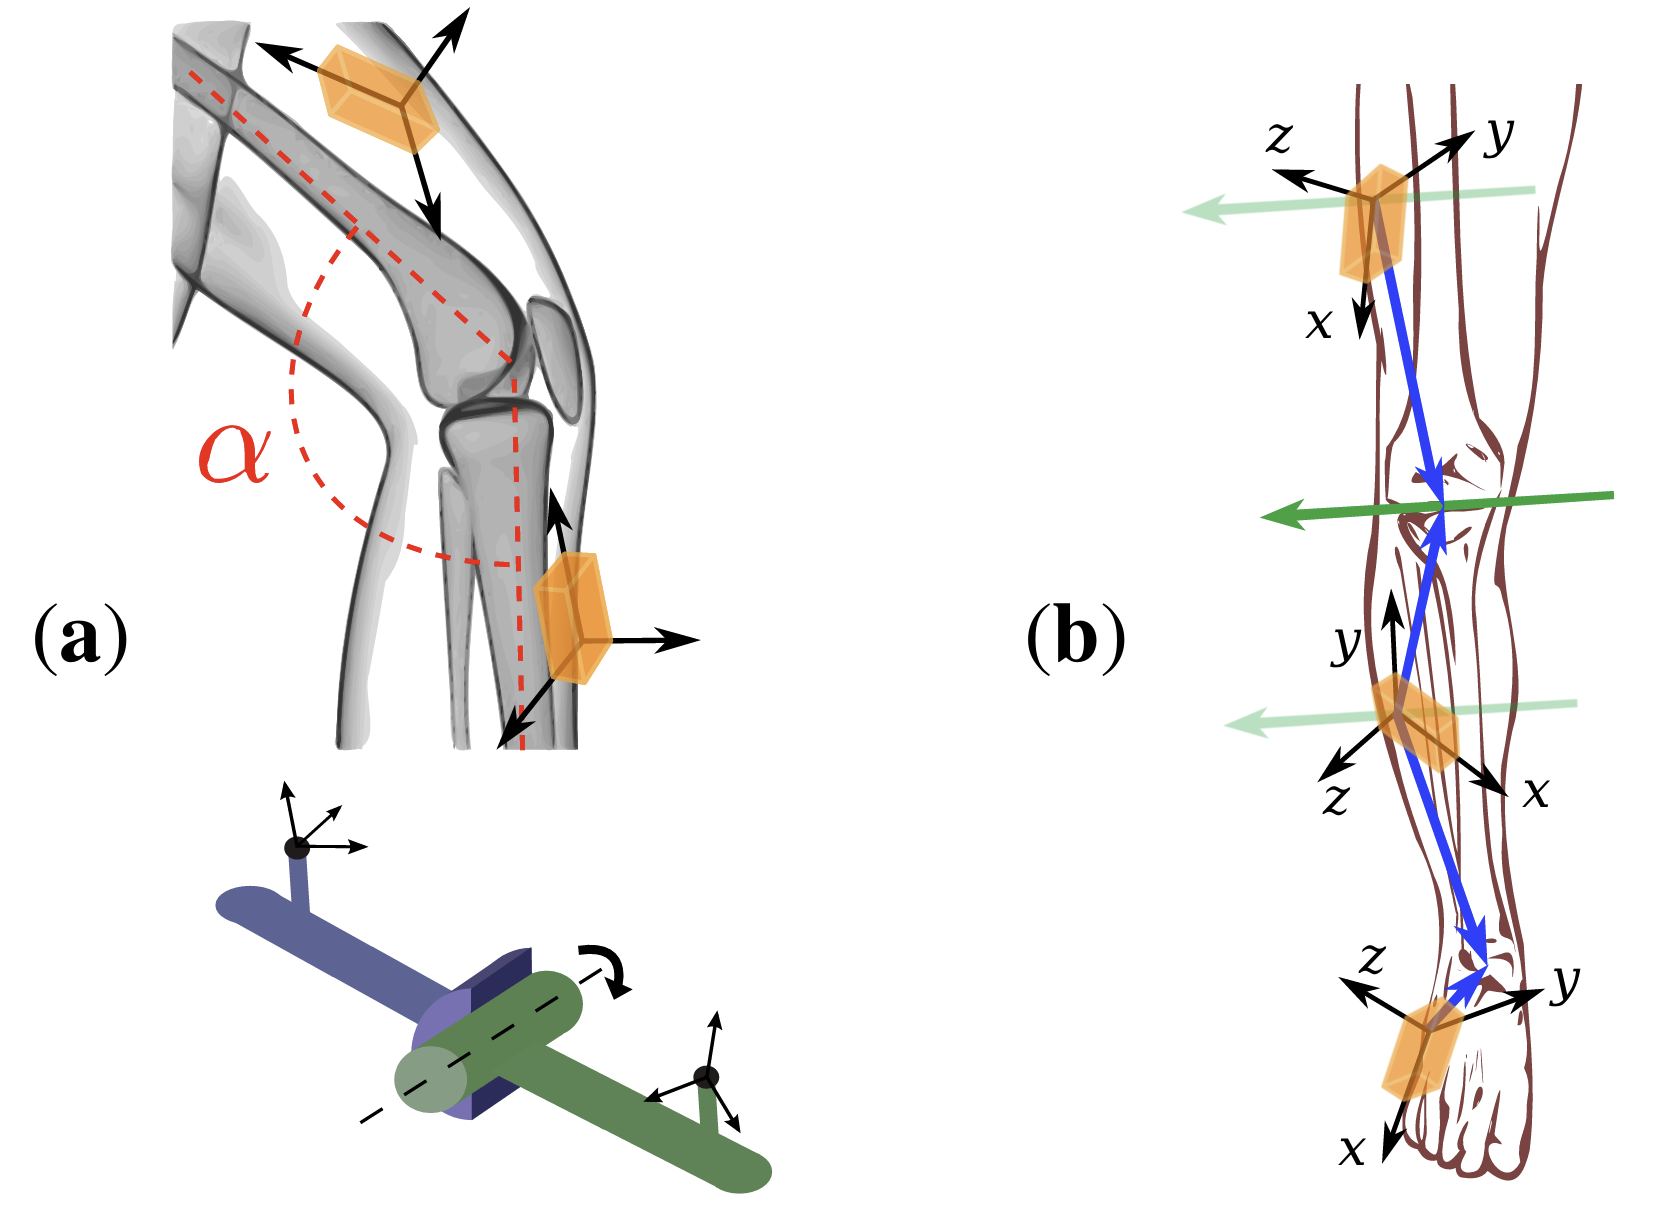
\includegraphics[width=0.75\linewidth]{images/kneeOrientation.png}
    \caption{\textbf{a)} Local sensor coordinate axes are not aligned with the physiological axes an dplanes by which the joing anvle, \(\alpha\), is defined \textbf{b)} The coordinates of the joint axis direction (green arrows) and the joint position (blue arrows) in the local coordinate system of the sensors \cite{seel_imu-based_2014}}
    \label{fig:enter-label}
\end{figure}

This issue is further compounded by the possible shifting of the IMUs over time. This poses issues since the initial offset between the IMUs is assumed to be accurately calibrated and constant throughout the session. Additionally the Madgwick filter is not capable of accounting for changes in sensor alignment over time, leading to possible inaccuracies if the IMUs are not secured well enough.

Another related challenge is the implicit assumption that the IMUs are do not experience significant external forces beyond those caused by the forward motion of the leg and gravity. In practice however, accelerometer readings can be affected by transient forces such as those that occur during foot strikes. These forces may introduce noise into the orientation estimation process, specifically in the correction step of the Madgwick filter, where accelerometer data is used to align the estimated gravity vector with the measured gravity vector.

Finally there is room for improvement with regards to the validation process itself. The Delsys derived knee angle, although likely more accurate than the In-House version since it has inbuilt sensor fusion algorithms for orientation estimation, is still using IMUs in order to estimate the angle. In order to benchmark in a better manner a goniometer sensor should be used instead or an even more robust sensor system. This could for example be the Xsens system used for validation of the open loop sequence which outputs knee angles without any additional processing necessary, but was regretfully not available during the period in which the knee angle estimation method was to be validated.. 

\subsection{Closed-Loop}

The results of the closed-loop gait control system provide an initial insight into the system's capabilities and limitations. The first issue is that of the difficulty of testing FES on healthy subjects, discussed earlier for the Open-Loop stimulation sequence.

The limited subject pool is another issue. Testing on a single subject restricts the generalizability of the results and does not account for individual variability. Differences in muscle composition, skin impedance and motor thresholds could significantly affect the control system's performance. A larger cohort of subjects would provide a more comprehensive understanding of the system's robustness.

Finally the delay and jagged IMU signal at faster speeds might indicate the limits of the system's control bandwidth at higher walking speeds. If the IMU signals do not manage to have a high enough accuracy to accurately measure the knee angle the closed loop control will introduce errors into the system that will make it in effect worse than the open loop implementation. The Madgwick filter has been proved to introduce very minimal delays, so this might indicate that the IMU sampling frequency might be insufficient to capture rapid movements accurately. 


%=================================================================
%                           End Document
%=================================================================
\end{document}